\documentclass{article}
\usepackage[utf8]{inputenc}
\usepackage{enumerate}
\usepackage{mathtools}
\usepackage{pdfpages}
\usepackage{titling}
\usepackage{pgfplots}
\usepgfplotslibrary[fillbetween]
\usetikzlibrary[patterns]
\usepackage{amsmath}
\usepackage{geometry}
\usepackage{subcaption}
\usepackage{graphicx}
\usepackage{stfloats}

\geometry{
  left=2cm,
  right=2cm,
  bottom=2cm,
  top=2cm
}

\setlength{\droptitle}{-10em}

\author{Magnus Moan}
\title{IT3708: Project 1}

\begin{document}

\maketitle

\hfill\\
\noindent
\textbf{Task 1} \\
I've chosen to implement my project in Java. My implementation is devided into three parts; model, controller and view. 
The model consists of 2 classes ({Board}, {Network}). 
The {Board} class defines a 10-by-10 playing board. The {Network} class defines a general neural network with inputs, outputs and weights. 
The controller part
of my implementation contains mechanisms for altering the model. The most important classes in the controller part are {Game}, {NeuralAgent}, {BaselineAgent} and
{MainApp}. The {Game} class controls the game by keeping count of number of rounds, number of games, score, etc. The most important procedures in this class are
\textit{play} and \textit{play\_one\_game\_without\_gui}. The agent classes defines the behavior of the different agents we are asked to implement. The {NeuralAgent} class
defines the behavior for all the agents associated with a neural network. Finally the {MainApp} class starts the entire application. 
The view part of the implementation is only considered with the graphical user interface of the application. A sample of the GUI can be seen on the next page.
\\[1ex]
My baseline agent have the following line of priority: food, empty, poison, wall. If my agent can choose between two or more options with the same item it will move forward before left
and left before right. My baseline agent recieves an average score of 20.579 on 1000 trials.
\\[1.5ex]
\textbf{Task 2} \\
See \textit{delta\_supervised} for code snippet where $\delta_i$ is calculated for supervised learning.
Comments in the code explains how the code implements equation 3. The argument $output\_index$ is the value $i$ from the equation.
\\[1.5ex]
\textbf{Task 3} \\
See \textit{delta\_reinforcement} and \textit{get\_best\_output\_from\_direction} for code snippet where $\delta_i$ is calculated for reinforcement learning.
Comments in the code explains how the code implements equation 5. The argument $output\_index$ is the value $i$ from the equation.
\\[1.5ex]
\textbf{Task 4} \\
See plot on next page. \\

\noindent
\textbf{Task 5} \\
Weights for the neural network after 100 rounds of training with the reinforcement neural network from task 3: \\
\begin{table}[h]
  \hspace{-1cm}
\begin{tabular}{l|cccc|cccc|cccc|}
\cline{2-13}
                              & \multicolumn{4}{c|}{Input: Left}     & \multicolumn{4}{c|}{Input: Forward}  & \multicolumn{4}{c|}{Input: Right}   \\ \cline{2-13} 
                              & Empty   & Wall    & Food   & Poison  & Empty  & Wall    & Food    & Poison  & Empty  & Wall    & Food   & Poison  \\ \hline
\multicolumn{1}{|l|}{Left}    & 2.2397  & -2.7783 & 3.5745 & -1.4320 & 0.9383 & 0.4935  & -0.7075 & 0.8791  & 0.3978 & 0.5686  & 0.0988 & 0.5373  \\ \hline
\multicolumn{1}{|l|}{Forward} & 0.63078 & 0.1547  & 0.6952 & 0.7466  & 2.3432 & -2.7790 & 3.8455  & -1.1820 & 0.6278 & 0.1805  & 0.7055 & 07136   \\ \hline
\multicolumn{1}{|l|}{Right}   & 0.3765  & 0.6160  & 0.4656 & 0.4675  & 0.7977 & 0.3024  & -1.808  & 1.0066  & 2.3271 & -2.7834 & 3.8259 & -1.4445 \\ \hline
\end{tabular}
\end{table}\\
We observe that the weights for each output is at its highest if there is food in the input corresponding to the same direction as the output. There are lesser values
for the other options in the inputs in the same direction as the output. We notice that the weights corresponding to inputs from the other directions are of lesser significance.
Below we see a sample of inputs and corresponding outputs (the direction corresponding to the highest output is chosen). 
\vspace{-1cm}
\begin{table}
\centering
\begin{tabular}{|ccc|ccc|c|}
\hline
\multicolumn{3}{|c|}{Input} & \multicolumn{3}{c|}{Output} & Chosen  \\ \hline
Left    & Forward  & Right  & Left    & Forward & Right   &         \\ \hline
Empty   & Wall     & Food   & 2.8321  & -1.4428 & 4.505   & Right   \\
Food    & Food     & Food   & 2.9658  & 5.2462  & 4.1108  & Forward \\
Poison  & Poison   & Empty  & -0.1550 & 0.1924  & 3.8011  & Right   \\
Wall    & Wall     & Poison & -1.7476 & -1.9107 & -0.5261 & Right   \\
Empty   & Empty    & Empty  & 3.5758  & 3.6017  & 3.5013  & Forward \\ \hline
\end{tabular}
\end{table}

\newpage
The agents in task 1, 2 and 3 performed close to the same average score. This is as expected as they recieve the same information from the sensors. The agent in task 4 recieved
more information and did therefore perform better compared to the others. See the graph showing average scores in the bottom of this page. 

\begin{figure}[h]
  \centering
  \begin{subfigure}{.5\textwidth}
    \centering
    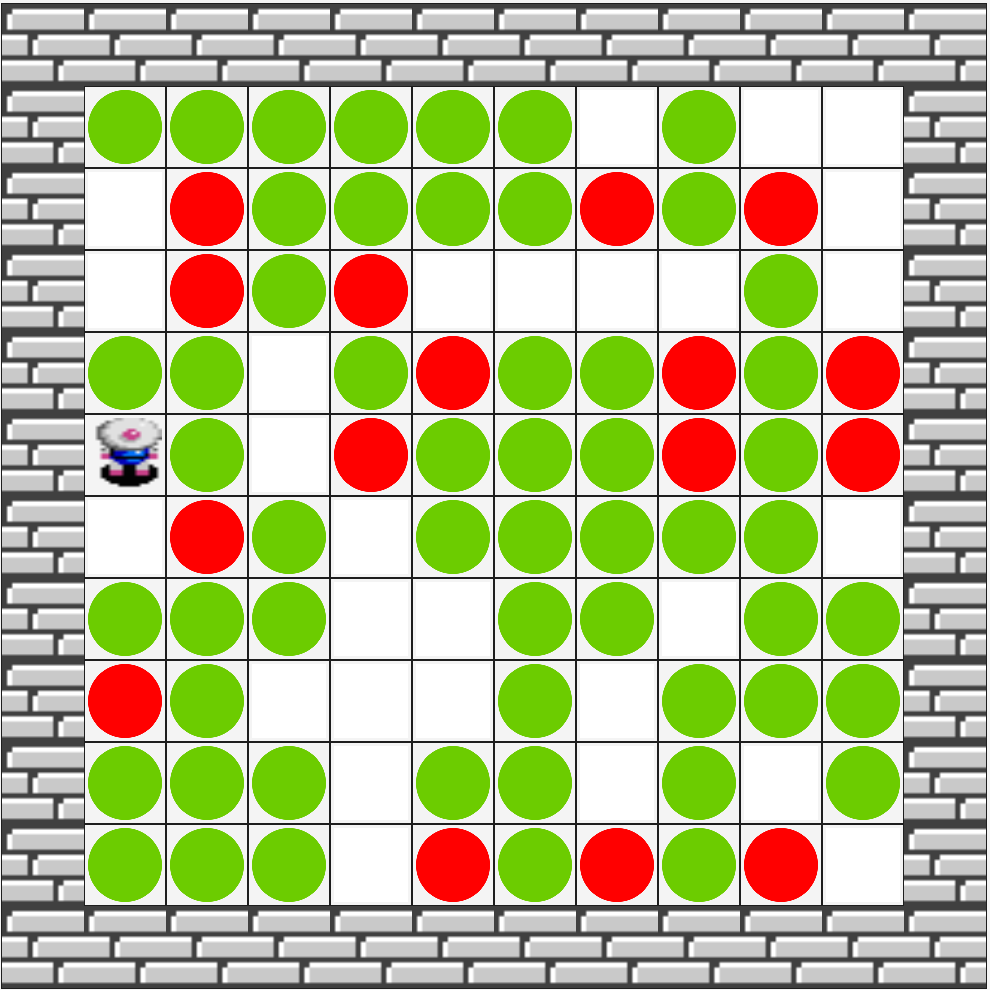
\includegraphics[scale=0.35]{png/flatland.png}
  \end{subfigure}%
  \begin{subfigure}{.5\textwidth}
    \centering
    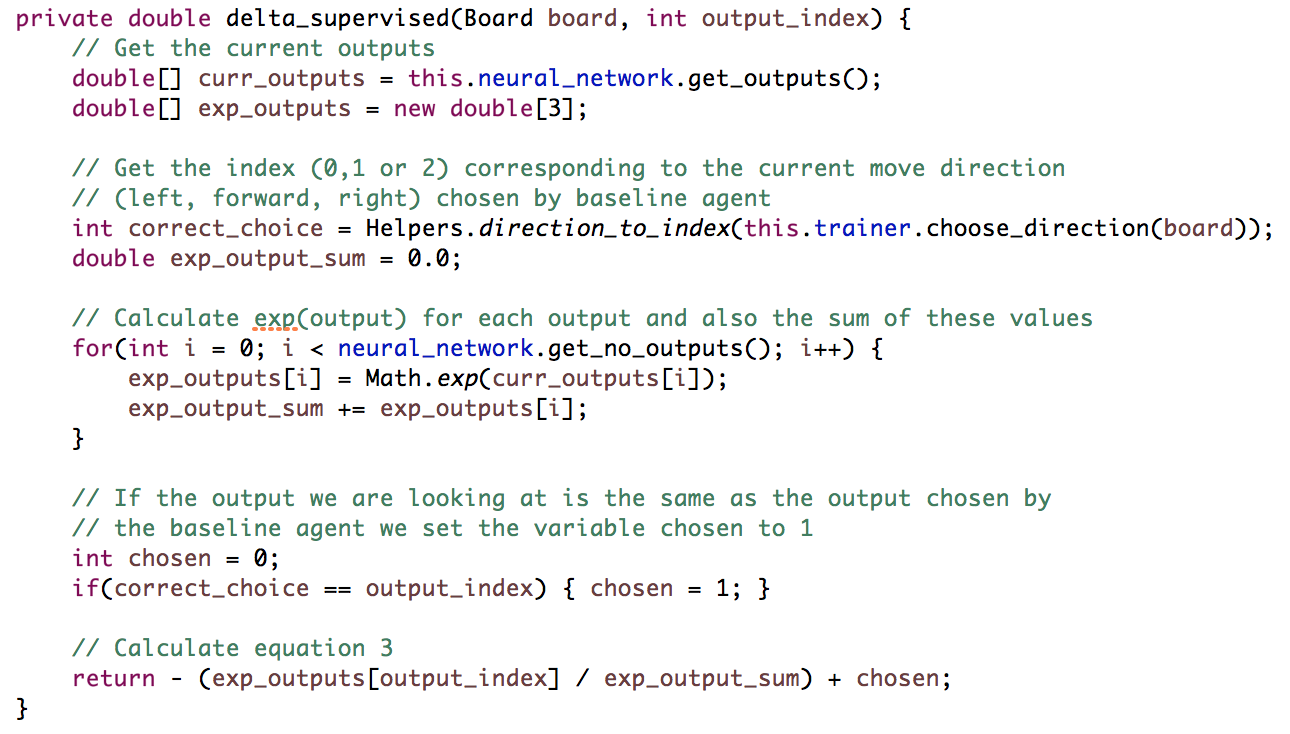
\includegraphics[scale=0.4]{png/delta_supervised.png}
  \end{subfigure}
\end{figure}

\begin{figure}[h]
  \centering
  \begin{subfigure}{.5\textwidth}
    \centering
    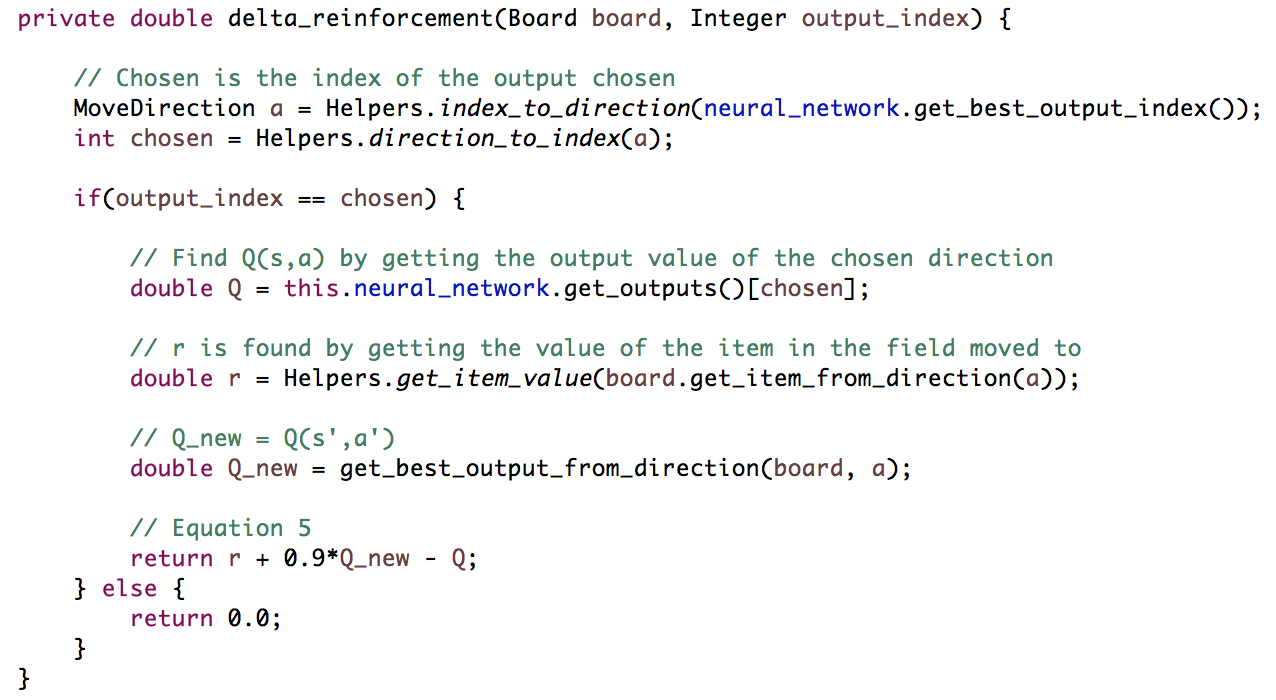
\includegraphics[width=1\linewidth]{png/delta_reinforcement.png}
  \end{subfigure}%
  \begin{subfigure}{.5\textwidth}
    \centering
    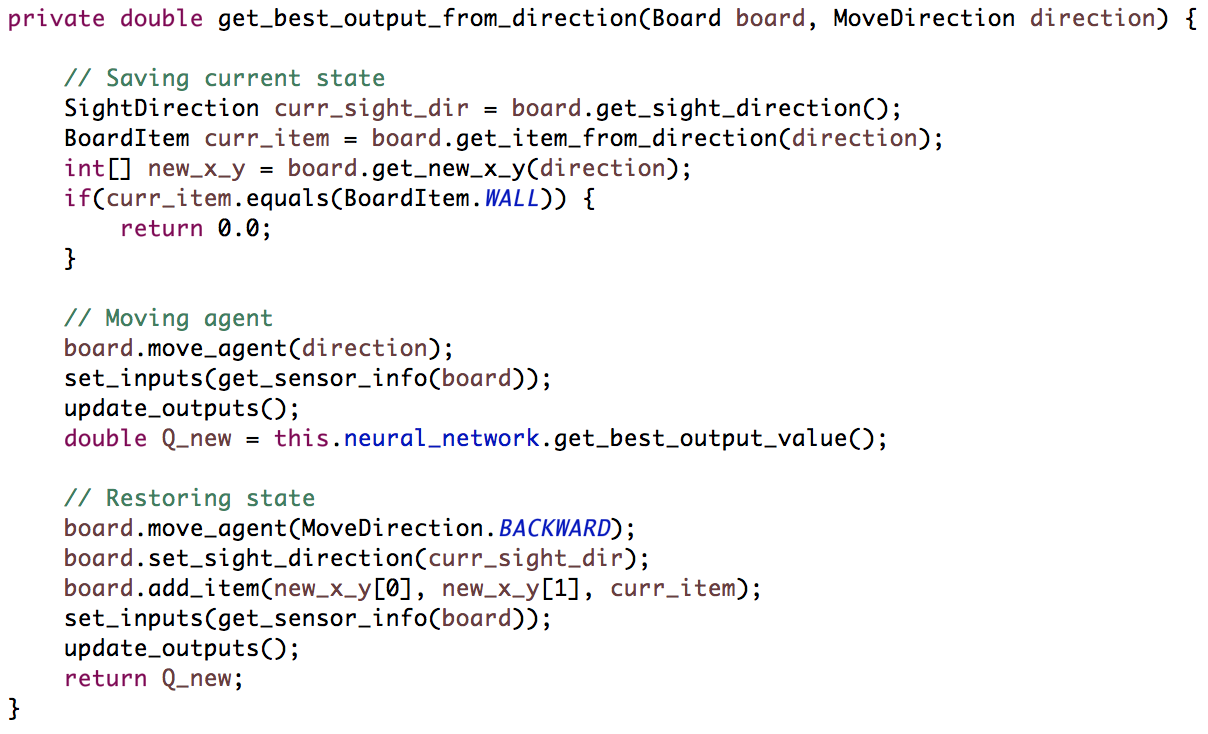
\includegraphics[width=1\linewidth]{png/q_new.png}
  \end{subfigure}
\end{figure}

\vspace{-1cm}

\begin{figure}[h!]
  \centering
  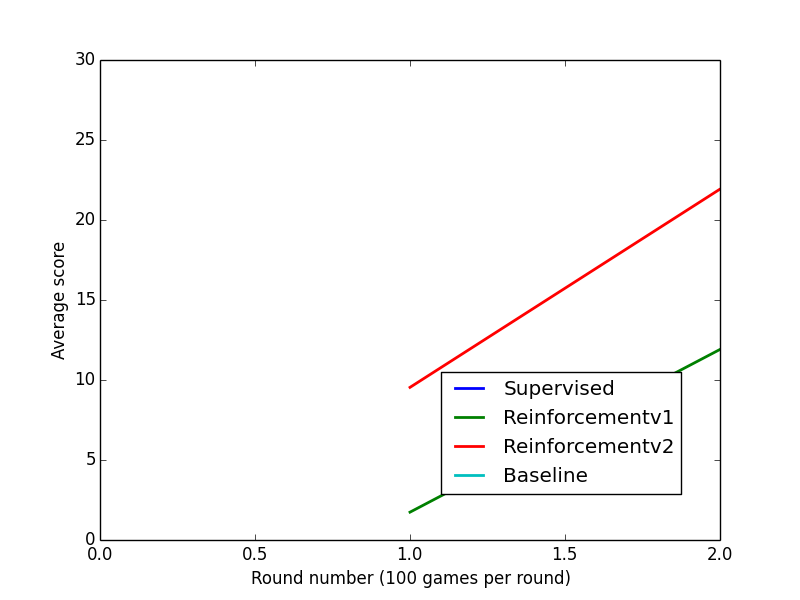
\includegraphics[scale=.5]{png/results.png}
\end{figure}

\end{document}
